\begin{table}[H]
\centering
\begin{tabular}{|l|l|l|l|l|}
\hline 
\textbf{Clasificación} & \textbf{Total} & \textbf{Aciertos} & \textbf{Errores} & \textbf{Eficiencia} \\
\hline
Estado & 1393 & 988 & 405 & 70.926 \\
\hline 
Categoría & 1393 & 770 & 623 & 55.276 \\
\hline 
\end{tabular}
\caption{Eficiencias generales con Hue 25-120}
\label{table:efficiency_general_25_120}
\end{table}

\captionsetup[figure]{skip=-10pt}

\begin{figure}[H]
\centering
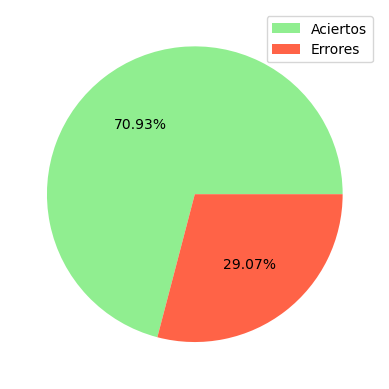
\includegraphics[scale=0.6]{images/result_global_state_25_120.png}
\caption{Eficiencia detectando el estado con Hue 25-120}
\label{img:efficiency_state_25_120}
\end{figure}

\begin{figure}[H]
\centering
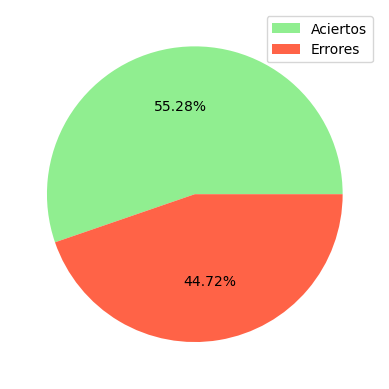
\includegraphics[scale=0.6]{images/result_global_class_25_120.png}
\caption{Eficiencia detectando la categoría con Hue 25-120}
\label{img:efficiency_category_25_120}
\end{figure}

\captionsetup[figure]{skip=10pt}

\begin{table}[H]
\centering
\begin{tabular}{|l|c|c|c|}
\hline 
\textbf{Categoría} & \textbf{Original} & \textbf{Calculado} & \textbf{Eficiencia} \\
\hline
healthy & 791 & 563 & 71.175 \\
\hline 
rust\_level\_1 & 344 & 175 & 50.872 \\
\hline 
rust\_level\_2 & 166 & 31 & 18.674 \\
\hline 
rust\_level\_3 & 62 & 0 & 0.0 \\
\hline 
rust\_level\_4 & 30 & 1 & 3.333 \\
\hline 
\end{tabular}
\caption{Eficiencia por categoría con Hue 25-120}
\label{table:efficiency_categories_25_120}
\end{table}

\begin{figure}[H]
\centering
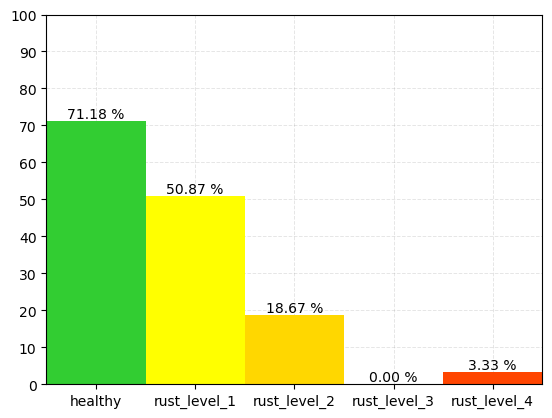
\includegraphics[scale=0.6]{images/result_classes_25_120.png}
\caption{Eficiencia por categoría con Hue 25-120}
\label{img:efficiency_categories_25_120}
\end{figure}
